% -*- program: pdflatex -*-
\documentclass[11pt,letterpaper,titlepage]{article}
\usepackage{evolution}
\usepackage[T1]{fontenc}
\usepackage{tgtermes}
\usepackage{etoolbox}
\hypersetup{
   pdftitle={Placeholder title for CVX-cactaceae Project Manuscript},
   pdfauthor={Alexa Tyszka, Karolis Ramanauskas, Boris Igi{\'c}}
   }
\usepackage[all]{hypcap}
\usepackage{doi}
\usepackage{graphicx}
%\graphicspath{{figures/}}
\renewcommand{\bibsection}{\section*{References}}
\providecommand{\e}[1]{\ensuremath{\times 10^{#1}}}
\newcommand{\ca}{\textit{ca}.}
\begin{document}
% TITLE =======================================================================
\title{\Large\bf{Placeholder title}}
\author{Alexa Tyszka$^{1}$, Karolis Ramanauskas$^{1,2}$ and Boris Igi\'{c}$^{1,3,4}$}
\date{
    $^1$Department of Biological Sciences\\
    University of Illinois at Chicago\\
    840 West Taylor St.\ MC067\\
    Chicago, IL 60607, U.S.A.\\
    [\baselineskip]
    $^2$Email: {\tt<kraman2@uic.edu>}\\
    $^3$Email: {\tt<boris@uic.edu>}\\
    $^4$Corresponding author.\\
}
\maketitle

%%%%%%NOTES%%%%%%

%%%%%%TODO%%%%%%

% No worries about warnings--we'll fix those later
% It _is_ important for the document to compile reliably (without errors)

%FIXMEs: 
% Read the log notes (git log) each time!
% Small stuff: Italicize all species binomials by convention: e.g., \texit{Schlumbergera truncata}. Not families, though! The convention helps with reading and whatnot, mainly it looks professional and it's a bit easier to read. Read sections on Scientific Nomenclature, Genes, and Viruses here: https://wwwnc.cdc.gov/eid/page/scientific-nomenclature
%Italicization done, 

% ABSTRACT ====================================================================
\begin{linenumbers}
\modulolinenumbers[1]
\setstretch{1.0}
\begin{abstract}
\textit{Potexviruses} (family Alphaflexiviridae ) are positive-sense single-stranded RNA viruses known to infect multiple species across plants, including species of \textit{Cactaceae}. 
\textit{Cactus Virus X, Zygocactus Virus X, Schlumbergera Virus X, Pitaya Virus X,} and \textit{Opuntia Virus X} are five of the 48 currently described \textit{Potexvirus} species, which all infect valuable ornamental and crop plants, often causing production losses. 
The taxonomic naming schemes often employ outdated plant name synonyms, complicating taxonomic assignments. Also, the source of infections in cultivated plants is unclear, as is the distribution of and significance of infections in wild species of cacti. 
The lack of clarity is partly related to low sampling across the family. 
Here, we report results of original RNA-seq experiments and archived sequence deposits, aimed at detecting \textit{Potexviruses} in cacti, assembling whole genomes, estimating their phylogenetic relationships, and delimiting viral species. 
The data suggests novel modes of transmission, based on expression analyses across tissues, particularly pollen. 
We also perform molecular evolutionary analyses to detect genomic regions under different modes of selection. 
Finally, we examine and discuss the implications of our analyses for the taxonomy of \textit{Potexviruses} across cacti.  

\end{abstract}


\setlength{\emergencystretch}{7.5pt}
\setstretch{1.0}
\setlength{\parindent}{0.25in}

\section*{Introduction}

The plant viriome represents a fundamentally complex evolutionary interaction between eukaryotic host and viral vector (\cite{delwart_viral_2007}). 
Plant viruses were the earliest characterized viruses, beginning with Mayer's publication on his discovery of \textit{Tobacco Mosaic Virus} in 1886 on tobacco plants (\cite{mayer1886mosaikkrankheit}) which followed Molisch's 1885 discovery of "protein bodies" on cacti: \textit{Schlumbergera truncata}, (previously \textit{Epiphylum truncatumin}) (\cite{molisch1885merkwurdige}). 
They may deserve to be called the first true purified viruses, but Molisch's "Proteinkörper" are absent from many reviews of historical virology (such as \cite{LECOQ2001929, lefeuvre_evolution_2019}).
Perhaps the most recent advancement in virology has been the of faster, cheaper, high-throughput environmental metagenomic techniques which have advanced many facets of evolutionary biology (\cite{delwart_viral_2007, lefeuvre_evolution_2019, schulz_towards_2017})
It has become evident through these discoveries that the greenhouse-raised and lab-grown organisms commonly analyzed in experiments actually represent a small fraction of living diversity. 
Metagenomic studies aim to sample hundreds of thousands of genomes, and have vastly expanded both the cellular tree of life (\cite{schulz_towards_2017, hug_new_2016}) and the viral tree of life (\cite{gregory_marine_2019, lefeuvre_evolution_2019, shi_redefining_2016}).  
Viruses display impressive morphological diversity and adaptations, many which allow them to infect plants (\cite{delwart_viral_2007, lefeuvre_evolution_2019}).
 Metagenomic analysis of plants, particularly understudied or non-crop plants have both enriched our genetic knowledge of plants and uncovered novel insights on viral evolution, adaptation, and transmission (Citations needed*). 
 A careful study of the plant viriome provides a view into underlying biological realities that are not currently understood.

The International Committee on Taxonomy of Viruses (ICTV) presently advises the taxonomy and approval of viruses (\cite{simmonds2017virus, lefkowitz2018virus,international2020new}).
The massive amounts of data resulting from metagenomic studies have caused significant revisions in ICTV policy (\cite{international2020new, simmonds2017virus}), but many viruses remain named by their host, location, or symptoms, all of which may cause confusion due to their overlap with other viruses.  
The Baltimore classification system attempts to standardize viral classification by intrinsic morphological characteristics of a virus' replication machinery, and has been integrated into the ICTV guidelines to better reflect viral evolutionary relationships \cite{international2020new}. 
The study of plant viruses particularly suffers from poor nomenclature due to the practice of naming a virus after a first discovered host which is subject to reclassification or renaming. 
The term "plant virus" in itself is problematic since there is strong evidence to suggest that viruses frequently spill over from fungal or invertebrate hosts to plants (\cite{lefeuvre_evolution_2019}).
Many agricultural plant viruses are also named for the common name of a plant, which carries its own problems, for example: \textit{Pitaya Virus X} is named for the common name "Pitaya" which can refer to as many as 31 species within the genus \textit{Selenicereus} (\cite{korotkova_phylogenetic_2017, guerrero_phylogenetic_2019, le_bellec_12_2011}). 
To complicate matters further, one virus may infect many hosts, and one host may contain many viruses. 
A single-stranded RNA virus has a faster rate of evolution than a host plant, and engages in different reproductive methods, making a direct comparison of virus-to-plant hosts difficult (citation needed).
There is no guarantee that viral evolution and speciation follows linearly behind plant evolution and speciation -- especially due to viral host-switching 
These problems persist throughout \textit{Potexvirus} and are especially prominent with regards to cactus-infecting \textit{Potexviruses}.
We suggest a phylogeny-based approach to remedy some prominent taxonomic issues within this specific clade that cause naming inconsistencies. 


%B: Hmmm, Intro is usually not allowed to have subsections. Also, Study System, Study Organism, or Study Site is commonly a subsection of Materials and Methods? Maybe, for reference, take a look at the organization of another paper? Karolis's paper is a good starting point, but any paper from a journal where you intend to send the ms is probably good, too.
%at: subsections removed.

% This subsection text, if in the M&M section should only be about the material that we are contributing. 
% If it is intended as background/review, those parts ought to be in the Introduction.
%at: I will trim this down soon and make it introduction-worthy.
\textit{Cactus Virus X}, \textit{Zygocactus Virus X}, \textit{Schlumbergera Virus X}, \textit{Pitaya Virus X}, and \textit{Opuntia Virus X} are all \textit{Potexviruses} (family Alphaflexiviridae) that are grouped broadly by their infections of certain cacti: \textit{Selenicereus undatus} and \textit{S. polyrhizus} (\cite{li_viral_2015, peng_molecular_2016}); \textit{Opuntia spp.} especially \textit{O. tuna} (\cite{koenig_molecular_2004, duarte_Potexvirus_2008}) and O. monacantha (\cite{attathom_occurrence_1978} Sammons 1961 Duarte 2008); \textit{Schlumbergera} (previously \textit{Zygocactus}) \textit{truncata} and \textit{S. bridgesii}  (\cite{duarte_Potexvirus_2008, koenig_molecular_2004}), \textit{Parodia }(previously \textit{Notocactus}) \textit{leninghausii }(\cite{park_detection_2018}),  \textit{Echinopsis chamaecereus f. cristata}, \textit{E. pectinatus f. cristata}, \textit{E. jusbertii}, and \textit{E. macrogona} (\cite{maliarenko_cactus_2013}); \textit{Mammillaria elongata f. cristata} (\cite{maliarenko_cactus_2013}); and multiple other species within many genera in the family Cactaceae (\cite{evallo_brief_2021}). 
Of these viruses, only\textit{ Cactus Virus X} (CVX) has been reported on wild \textit{Ferocactus cylindraceus }(previously \textit{Ferrocactus acanthodes}) (\cite{attathom_occurrence_1978}) although this report predates DNA records confirming the viral identity. 
Additionally, although they are originally found on cacti, the viruses are frequently manipulated with serological experiments and have been found to produce lesions (which indicate infection) on: Chenopodium murale L. (\cite{maliarenko_cactus_2013}) and C. quinoa (\cite{attathom_identification_1978,attathom_occurrence_1978, brandes_untersuchungen_1963-1}; Nicotiana alata Link el. Otto (\cite{maliarenko_cactus_2013}); Four species of Amaranthaceae (\cite{attathom_identification_1978}); Escobaria vivipara (\cite{attathom_identification_1978}); and other cactaceae (\cite{attathom_identification_1978}). 
All cactus-infecting \textit{Potexviruses} consist of roughly 6,600 bp of positive-sense single-stranded RNA. They have similar rod-shaped filamentous virions and share the same division of five primary open reading frames (ORFs): Replicase (Rep), Triple gene block (TGB), Coat protein (CP), coded in the 5' direction as well as two smaller overlapping ORFs coded in the 3' direction: ORF6 and ORF7 (\cite{evallo_brief_2021,liou_complete_2004, martelli_family_2007}). 
They are closely related to other \textit{Potexviruses} such as \textit{Alternantha Mosaic Virus} and \textit{Papaya Mosaic Virus} (\cite{martelli_family_2007, park_detection_2018, liou_complete_2004}). 
These viruses produce a wide range of symptomatic and damaging infections in cacti. 
Reports of symptomatic plants range from 5.5 percent of wild \textit{Ferocactus cylindraceus} (\cite{attathom_occurrence_1978}) up to 44 percent of crop plants on Hainan Island, China (\cite{peng_molecular_2016}). 
However, many infected plants do not show external signs of viral infection (\cite{liou_complete_2004, bos_symptoms_1977}). 
The most commonly recognized symptoms of disease are mosaic, mottling, stunted growth and distortion (\cite{maliarenko_cactus_2013, peng_molecular_2016, attathom_occurrence_1978}). 
It is yet unclear what the method of transmission from infected plant to new host is. 
Some reports specify that cactus-infecting \textit{Potexviruses} can only be transmitted through grafting (\cite{duarte_Potexvirus_2008, martelli_family_2007}) but most agree that transmission can occur through other mechanical contact such as sap inoculation (\cite{liou_complete_2004, maliarenko_cactus_2013, park_detection_2018}) and external tissue contact. 
Grafting is a primary means of propagation among crop cacti (\cite{park_detection_2018}), and \textit{Selenicereus} is a commonly chosen graft stock. 
However, there are reports of other members within the family \textit{Alphaflexiviridae} transmitting via insect and seed vectors (\cite{martelli_family_2007}), and pre-DNA studies tentatively suggest that \textit{CVX} may transmit via pollen in the wild (\cite{attathom_occurrence_1978}).

Knowledge about cactus-infecting \textit{Potexviruses} contributes to a growing yet biased study of plant viruses. 
The evolutionary history of these viruses is obscured due to human-assisted dispersal, grafting, and cultivation, which parallels the disproportionate sampling representation of plants raised in greenhouses or for agricultural production. 
However, \textit{Cactus Virus X} and associated viruses seem restricted to cactaceous hosts for unknown reasons -- every sample of CVX or CVX-related viruses has come from cacti. 
A wild origin has not been definitively identified, and the few studies that have investigated wild \textit{Potexviruses} of cacti predate DNA methods.
Recent sequencing efforts have revealed multiple inconsistent virus-host pairs on cacti. 
Although many metagenomic studies capture environmental genetic information that allows for virus identification, these may be biased due to tissue type and expression rates of viruses (\cite{lacroix2016methodological}). 
The pursuit of wild cactus-infecting \textit{Potexviruses} serves to expand our evolutionary knowledge of viral evolution, host selection, and transmission mechanics. 
The relationships of the virus can be investigated with a thorough phylogenetic approach, using available virus samples. 
In this study we present the largest to date phylogeny of cactus-infecting Potexviruses. 
We attempt to use this expanded phylogeny to answer relevant questions about Potexvirus evolutionary relationships as well as revisiting the utility of decades-old taxonomy in current virus research. 


% METHODS ====================================================================
%------------------------------------------------------------------------------
\section*{Materials and Methods}
%------------------------------------------------------------------------------

\subsection*{Study Organism}


\subsection*{RNA Sequencing}

Tissues were collected and immediately submerged in 1.5 ml of RNA\textit{later}\texttrademark~solution (Invitrogen).
Submerged samples were generally held at room temperature for thirty minutes and then stored at -80$^{\circ}$C.
Approximately 100 mg of tissue was ground with a cooled mortar in 1.5 ml tubes.
Total RNA was isolated using Total RNA Mini Kit (Plant kit; IBI Scientific, Cat. No. IB47341) following manufacturer's instructions.
We assessed RNA concentration and purity with a NanoDrop\texttrademark~Lite Spectrophotometer (Thermo Scientific).
The twenty-three samples used in this study were sequenced as part of a larger sequencing effort which consisted of four separate sequencing runs and included additional samples from other plant species.
Sequencing libraries were prepared using the KAPA Stranded mRNA-Seq (Roche), and these libraries were sequenced on a single lane of Illumina \mbox{HiSeq}~4000 or Illumina \mbox{NovaSeq}~6000 platform (paired-end 150 bp reads) at the Duke University Center for Genomic and Computational Biology.
The number of resulting read pairs (for the twenty-three samples presented here) ranged from 4,148,932 to 9,618,084 with a median of 6,363,556 and average of 6,293,553 (Table~S1).

\subsection*{RNAseq Assemblies}

Raw paired-end Illumina reads were first processed using \mbox{Rcorrector}~v1.0.4 \cite{song2015} to correct for random sequencing errors.
Then, reads were trimmed with \mbox{Trimmomatic}~v0.39 \cite{bolger2014} to remove any read containing bases with Phred scores lower than 20, low quality reads less than 50 bp long, and any adapter or other Illumina-specific sequences that were still present.
The remaining reads were filtered with \mbox{Kraken}~2 \cite{wood2019} to remove Small and Large Subunit ribosomal RNA (SILVA database) \cite{quast2013} and contaminating reads (minikraken2\_v2 database).
Additionally, we used custom-built databases, derived from RefSeq libraries: UniVec\_Core, viral, mitochondrion, plastid, plasmid, archaea, bacteria, protozoa, human, and fungi to minimize the number of contaminating and non-nuclear reads.
Only paired reads were used for transcriptome assemblies.
\textit{Schlumbergera truncata} filtered reads were combined across all samples into a single RNA-seq data set.
We conducted a \textit{de novo} transcriptome assembly using \mbox{Trinity}~v2.8.5 \cite{grabherr2011} to generate a single reference transcriptome assembly for \textit{Schlumbergera truncata}.
The same assembly protocol was followed for the single pistil sample of \textit{Matucana madisoniorum}.

\subsection*{NCBI Data Collection and Compilation}
We collected publicly available genomes, complete proteins, gene annotations, and available metadata from Potexviruses (NCBI:txid12176) (NCBI: www.ncbi.nlm.nih.gov/, accession numbers provided in Supplemental Data). 
The untranslated regions (UTRs) were trimmed from the sequences to provide consistency.


We also searched the NCBI Sequence Read Archive (SRA) database (www.ncbi.nlm.nih.gov/sra) for RNA-sequencing (RNA-seq) data within Caryophyllales (NCBI:txid3524) that had been sequenced using the Illumina library sequencing platform. 
For each identified SRA run accession (SRR), any viral RNA that matched sample cactus-infecting Potexvirus RNA (accession numbers provided in Supplemental Data) was identified, extracted, and assembled using the kakapo 0.7.3-dev pipeline (http://flightless.one) with Kraken2 viral filters disabled. 
The .sam files produced through kakapo were loaded through Geneious 11.1.5 along with the Schlumbergera reads.
%KR check
These sequences were annotated using the Geneious 11.1.5 "Find ORFs" function. 

The complete dataset comprises: 37 existing Potexvirus genomes and proteins, 4 new viral sequences located within original Schlumbergera truncata RNA-seq data, and 52 viral sequences found within NCBI Caryophyllales RNA-seq data.

\subsection*{Sequence Alignment and Phylogenetic Analyses}
Sequence alignments were performed through MAFFT v7.429 (\cite{katoh_mafft_2002}) using the full dataset.
%KR check
The aligned sequences were divided by ORF using the annotations to produce five partial sequence alignments corresponding to each ORF to accompany the full-sequence alignment. 
The individual proteins were exported to .FASTA files, then gaps at the start of the sequence and stop codons were removed manually. 
Phylogenetic relationships and bootstrap values were inferred using IQtree v1.6.12 (\cite{nguyen_iq-tree_2015}), ModelFinder (\cite{kalyaanamoorthy_modelfinder_2017}), and UFBoot (\cite{hoang_ufboot2_2018}) for both the individual gene/protein alignments and the full sequence alignment. 
Trees were visualized in R version 4.0.3 using ggtree v2.4.2 (\cite{yu_ggtree_2017}). 
Host information was obtained through reported metadata and mapped onto the phylogeny. 
Species groupings were determined using the existing species boundaries when compared to the phylogenetic branch lengths within the Potexvirus genus. 
This was generally consistent with most recent branch lengths over 0.1 subs/site and this value was therefore used as a cutoff. 
Pairwise distance analysis was conducted on the sequence alignments in R using the ape v5.5  dist.dna() function with a raw model. 
For each defined clade, nonzero pairwise distances between each possible combination of tips was averaged. 
Expanded phylogenetic trees and individual gene/protein trees are available in the Supplementary Data.
Pistils (without ovaries), pollen, leaf, and root tissues were collected and immediately submerged in 1.5 ml of RNA\textit{later}\texttrademark~solution (Invitrogen).
Submerged samples were held at room temperature for thirty minutes and then moved to a -80 C freezer for storage.
Approximately 100 mg of tissue was ground to a fine powder in 1.5 ml tubes submerged in liquid nitrogen.
Total RNA was isolated using Total RNA Mini Kit (Plant kit; IBI Scientific, Cat. No. IB47341) following manufacturer's instructions.
We assessed RNA concentration and purity with a NanoDrop\texttrademark~Lite Spectrophotometer (Thermo Scientific).
The XX samples used in this study were sequenced as part of a larger sequencing effort which consisted of XXX separate sequencing runs and included additional samples from other plant species.
Sequencing libraries were prepared using the KAPA Stranded mRNA-Seq (Roche), and these libraries were sequenced on a single lane of Illumina \mbox{HiSeq}~4000 or Illumina \mbox{NovaSeq}~6000 platform (paired-end 150 bp reads) at the Duke University Center for Genomic and Computational Biology.
The number of resulting read pairs (for the XX samples presented here) ranged from X,XXX,XXX to X,XXX,XXX with a median of X,XXX,XXX and average of X,XXX,XXX (Table~S1).


%------------------------------------------------------------------------------
\section*{Results and Discussion}
%------------------------------------------------------------------------------
\subsection*{Characterization}
The collection of \textit{Schlumbergera} samples and thorough investigation of previously published data on Cactaceae resulted in the discovery of XX new virus lineages.
These were all consistent with published genomic \textit{Potexvirus} data.
The newly discovered viruses from \textit{Schlumbergera} were generated as consensus sequences of XX individual reads which reliably recovered XX percent of the published\textit{ Cactus Virus X }genome. 
For the newly discovered viruses with \textit{Selenicereus} hosts, the XXX sample reads recovered XX percent of the \textit{CVX} genome.
All of the publicly available new viral lineages were discovered on \textit{Selenicereus} hosts.
We were able to reliably annotate the open reading frames of the viruses to recover all known Potexvirus proteins.

\subsection*{Distribution of Genetic Distances}
Pairwise distances between species were calculated for six groups, with a value of 0 indicating identical sequences and a value of 1 indicating completely divergent sequences (Figure 2). 
The average nonzero pairwise distance between all included Potexvirus tips was 0.256, maximum = 0.4925. 
When the outgroup (including Plantago asiatica MV, Alternantha MV, Papaya MV, etc.) was excluded from pairwise analysis, the average nonzero pairwise distance value was 0.177, maximum = 0.326. 
When these cactus-infecting Potexviruses were subdivided into six groups of relatively recent diversification, the average nonzero pairwise distance for full-genome sequences was always above 0.015. 

For the genes RNA-dependent RNA polymerase (RdRp) and Coat protein (CP), which the ICTV recommends be analyzed for species delimitation, the average nonzero pairwise distance was always  above 0.02 (Figure 2). 
This correlates to roughly greater than 97.5 and 98 nucleotide identity. 


\subsection*{Phylogenetic Relationships}
The phylogenetic tree places the new viral sequences from Schlumbergera and Selenicereus near existing viral species within Potexvirus (Figure 1). 

The S. truncata samples were located within the Cactus Virus X clade and appear to represent the only known discovery of Cactus Virus X on members of Schlumbergera. 
The publicly available data which was collected from NCBI produced 52 new viral sequences which were dispersed among viral species. 
These samples were exclusively representative of Selenicereus undatus and Selenicereus polyrhizus hosts. 
The Cactus Virus X species clade is expanded by a factor of 8. 
The only putative species that was not expanded by either the Schlumbergera data or the Selenicereus data was Opuntia Virus X, which appears to be an outgroup to the other cactus-infecting Potexviruses. 

\subsection*{Recombination and selection analysis}
\subsection*{Grouping}
The species within the phylogeny appear to be generally characterized by long (*) branch lengths separating clusters of closely related (short branch lengths) tips. 
Cactus Virus X appears to have two time-separated evolutionary distant sets of tips. 
These have been marked as different colors in Figure 1. 

\subsection*{Concluding Remarks}

%------------------------------------------------------------------------------
\section*{Acknowledgments}
%------------------------------------------------------------------------------

Acknowledgments text.

% BIBLIOGRAPHY ================================================================
\pagebreak
\raggedright{}
\setstretch{1.0}
\setlength{\parindent}{0.0in}
\bibliographystyle{evolution}
%{\fontsize{10pt}{15pt}\selectfont
\bibliography{cvx-refs}
%}
\end{linenumbers}
% FIGURES =====================================================================
\pagebreak
\frenchspacing
\setstretch{1.0}
\setlength{\parindent}{0.0in}

\section*{Figures}


 \begin{figure}[ht]
 \centering
 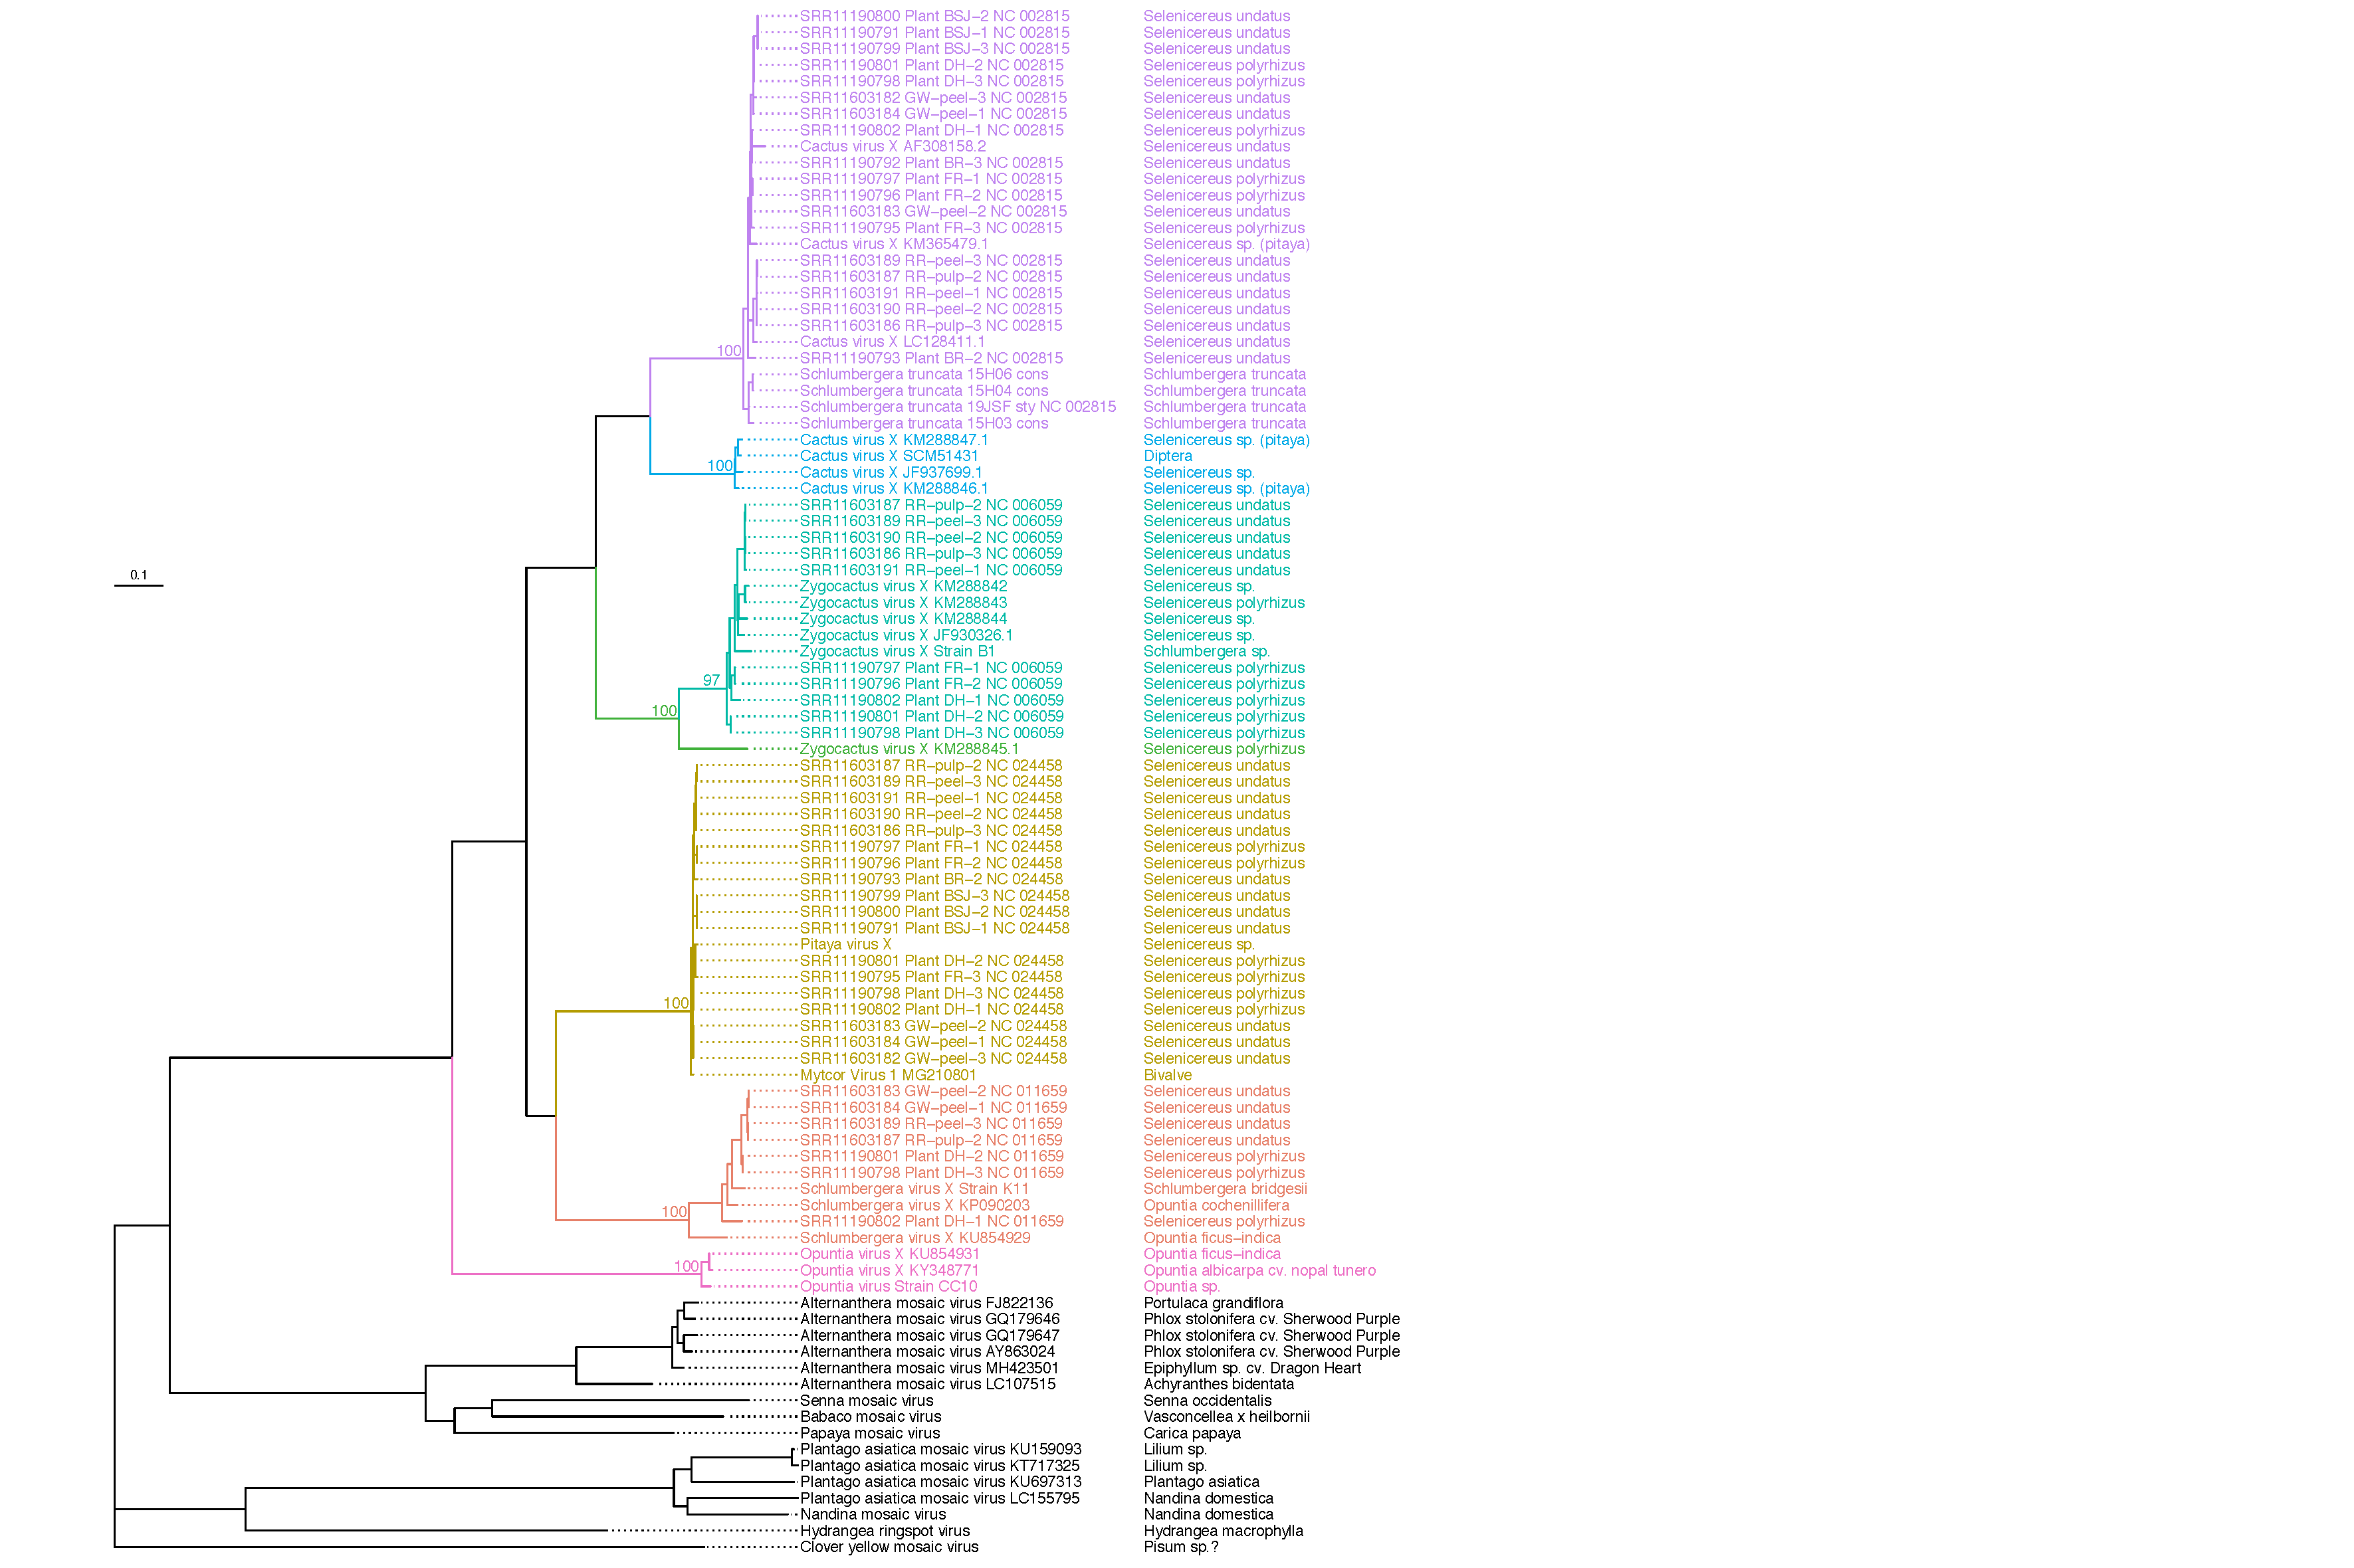
\includegraphics[width=0.5\linewidth]{../images/full_bootstrap_tree.pdf}
 \begin{NoHyper}
 \caption{{\fontsize{10pt}{11pt}\selectfont}
 \label{Phylogeny}
 \end{NoHyper}
 \end{figure}

% \begin{figure}[ht]
% \centering
% \includegraphics[width=0.5\linewidth]{FILE_PATH}
% \begin{NoHyper}
% \caption{{\fontsize{10pt}{11pt}\selectfont
% \label{fig:FIG_LABEL}
% \end{NoHyper}
% \end{figure}

% END =========================================================================

\end{document}
